\chapter{Adaptive Model Predictive Control for Trajectory Planning} \label{sec:chaser_ampc}
Rendezvous deals with the approach of the chaser from a farther location to a location close to the target.
Due to the uncertainty of orbital dynamics as a result of factors such as the elliptical nature of the orbit, electromagnetic fluctuations, atmospheric drag, and solar radiation, we propose the application of adaptive model predictive control to plan the trajectory of the chaser for rendezvous with the target.
While it is a common assumption to consider a circular orbit, this introduces an error in the dynamics of the chaser.
This further causes uncertainty even when the orbit is considered to be elliptical with an incorrect value for its eccentricity.
The dynamics of the chaser in such an orbit can be modeled using the Tshauner-Hempel equations \cite{yamanaka2002new,sinclair2015geometric}.
We also consider the effect of non-conservative forces such as quadratic atmospheric drag \cite{carter2002clohessy} on the target and the chaser which can be represented using the drag constants of the spacecraft.
We propose formulating these quantities as unknown parameters in the problem that can be learned over time based on the error in the estimated state of the chaser, $\hat{\boldsymbol{r}}$, with respect to its actual state, $\boldsymbol{r}$.
For this purpose, the chaser implements adaptive model predictive control (AMPC) wherein it plans trajectories and updates the calculated trajectory at regular intervals while also updating the estimates for the unknown quantities.

\section{Trajectory Planning} \label{ssec:rendezvous-traj-planning}
The rendezvous trajectory planning problem involves generating trajectories such that the goal state is on a sphere around the target, i.e., at a fixed predetermined distance from the target.
While the minimum possible goal radius is defined by the size and shape of the target (ref. Section \ref{sec:rendezvous-collision-constraints}), multiple intermediate spheres may be used for better observation and inertial estimation of the target.
Hence, the trajectory planning problem for rendezvous can be formulated as the following optimization problem:
\begin{align}
    \min_{\boldsymbol{r}, \boldsymbol{u}}\ J(\boldsymbol{r},\boldsymbol{u})&=h(\boldsymbol{r}(\theta_f))+\int_{\theta_0}^{\theta_f} \left((\boldsymbol{r}-\boldsymbol{r}_f)^TQ(\boldsymbol{r}-\boldsymbol{r}_f)+\boldsymbol{u}^TR\boldsymbol{u}\right)d\theta
\end{align}
\addtocounter{equation}{-1}
\vspace{-4ex}
\begin{subequations}
\begin{align}
    \textrm{s.t. } & \boldsymbol{r}'=A(\theta)\boldsymbol{r}+B\boldsymbol{u}+\boldsymbol{d}(\theta),\hspace{8em}\\
    & \boldsymbol{r}(\theta_0)=\boldsymbol{r}_0,\quad\boldsymbol{r}\in{\mathcal{C}}_R,\label{eqn:radial-limit-constraint}\\
    & \boldsymbol{v}\in{\mathcal{V}},\quad\boldsymbol{u}\in{\mathcal{U}},
\end{align}
\end{subequations}
where $\boldsymbol{r}^T=\left[\boldsymbol{p}^{T},\ \boldsymbol{v}^{T}\right]$ is the state of the system consisting of its position $\boldsymbol{p}$ and velocity $\boldsymbol{v}$ such that the system dynamics are given by the extended Tshauner-Hempel equations (explained in Appendix \ref{app:ellp-undrag}), $\boldsymbol{r}_0$ represents the starting point of the chaser, final state cost function $h(\boldsymbol{r}(\theta_f))$ is minimized to move closer to the target, and ${\mathcal{V}}$ and ${\mathcal{U}}$ represents the set of permissible velocities and control inputs of the chaser.
The additional non-convex radial-limit constraint in Equation \ref{eqn:radial-limit-constraint} ensures that the chaser remains outside all possible locations of the target, hence avoiding collisions.
As a result, the set of feasible locations is defined as ${\mathcal{C}}_R$.
This is described in detail in Section \ref{sec:rendezvous-collision-constraints}.

Docking is the final process of attaching the chaser to the target after the chaser has reached close proximity.
This is identical in structure and dynamics to rendezvous.
However, in order to make physical contact feasible, the collision constraints are modified with consideration of the physical (such as the angular velocity) and inertial (such as the moment of inertia) parameters of the target.
As a result, the radial-limit constraint is replaced by a target-limit constraint $\boldsymbol{r}(\theta)\in{\mathcal{C}}_D$ such that the chaser does not collide with the target.
Moreover, the final state cost function is made stricter to achieve docking with the target.
Additionally, to prevent plume impingement, the permissible control input set ${\mathcal{U}}$ can be made stricter \cite{starek2017fast}.
We do not consider this in this paper but propose using this approach in practice.

\section{Rendezvous and Docking Constraints} \label{sec:constraints}
\subsection{Time-Varying Final State Constraint}
\label{sec:time-varying-final-state-constraint}
Although the docking position is fixed relative to the target, it is rotating in the LVLH frame.
As a result, we incorporate a time-varying final state heuristic $\zeta(\boldsymbol{r}(\theta_f))$ such that the chaser tracks and attaches to the target at a set docking point.
The upper bound of this heuristic is decreased sequentially in the rendezvous operation to emulate observation spheres.
On the other hand, to facilitate docking, this heuristic is set to zero for docking.
Let the desired docking point be represented as $\left.\boldsymbol{\rho}_{\theta_f,T}\right|_{\theta_T=0}$ for when the target is at no rotation.
The final state heuristic can be defined using the Newton-Euler equations as follows:
\begin{align}
    \boldsymbol{\theta}_T(\theta)&=\begin{bmatrix}\alpha_T(\theta)&\beta_T(\theta)&\gamma_T(\theta)\end{bmatrix},\\
    \dot{\boldsymbol{\theta}}_T(t)&=\boldsymbol{\omega}_T(t),\\
    I\dot{\boldsymbol{\omega}}_T(t)&=-\boldsymbol{\omega}_T(t)\times I\boldsymbol{\omega}_T(t) + \boldsymbol{\tau}_T(t),\\
    \zeta(\boldsymbol{r}(\theta_f))&=\boldsymbol{r}(\theta_f)-\left.R(\theta_f)\boldsymbol{\rho}_{\theta_f}\right|_{\theta_T=0},
\end{align}
where $R(\theta_f)$ is the rotation matrix at the final true anomaly $\theta_f$ (we consider all angles to be described using Tait-Bryan rotations), $\boldsymbol{\tau}_T(t)=0$ until the end of docking, and time $t$ and true anomaly $\theta$ are interchangeable using the relations given in Section \ref{sec:relevant-knowledge}.

For rendezvous, we bound this final state heuristic by a positive ``radius" since it is not feasible to reach the final state while operating under the time-invariant rendezvous collision constraint (explained in Section \ref{sec:rendezvous-collision-constraints}).
This gives us the final state cost for rendezvous as follows:
\begin{equation}
    \label{eqn:rendezvous-cost}
    h(\boldsymbol{r}(\theta_f))|_{\text{rdv}}=Q_\text{rdv}\max{\left(||\zeta(\boldsymbol{p}(\theta_f))||-r_R, 0\right)}.
\end{equation}
For docking, we define the final state cost so that this heuristic approaches zero at the final true anomaly:
\begin{equation}
    h(\boldsymbol{r}(\theta_f))|_{\text{dkg}}=Q_\text{dkg}\zeta(\boldsymbol{p}(\theta_f)).
\end{equation}
\subsection{State and Input Bounds}
\label{sec:state-input-bounds}
Given the general definition for state and input bounds, \cite{brett2019dynamic}
\begin{align}
    ||P_{\boldsymbol{r}}\boldsymbol{r}+q_{\boldsymbol{r}}||&\leq C_{\boldsymbol{r}},\\
    ||P_{\boldsymbol{u}}\boldsymbol{u}+q_{\boldsymbol{u}}||&\leq C_{\boldsymbol{u}},
\end{align}
we define the following permissible state and input sets:
\begin{align}
    \boldsymbol{p}&\in{\mathcal{P}}:=\{\boldsymbol{p}\ |\ |p_i|<    \infty\},\quad\text{(no bound)}\\
    \boldsymbol{v}&\in{\mathcal{V}}:=\{\boldsymbol{v}\ |\ |v_i|\leq C_{V}\},\\
    \boldsymbol{u}&\in{\mathcal{U}}:=\{\boldsymbol{u}\ |\ |u_i  |\leq C_{U}\},
\end{align}
for each dimension $i=1,2,3$, where $C_{V}$ and $C_{U}$ are constants.
\subsection{Rendezvous Collision Constraints}
\label{sec:rendezvous-collision-constraints}
We define rendezvous to be necessarily bounded outside the positional limits of the target.
As a result, we constrain the chaser from entering a minimal sphere that completely bounds the target.
Since the sphere is a cyclically symmetrical shape in all directions, the rotation of the target does not affect its shape or size and, hence, the constraint is time-invariant, reducing computational complexity for the rendezvous problem.
Therefore, the rendezvous collision constraint can be written as $\boldsymbol{r}\in{\mathcal{C}}_R$ where:
\begin{equation}
    {\mathcal{C}}_R:=\{\boldsymbol{r}\ |\ ||\boldsymbol{p}||>\rho_T, \rho_T=\min\rho \text{ s.t. } ||\boldsymbol{p}_T||\leq\rho\ \forall\ \boldsymbol{p}_T\in\text{T}\}.
\end{equation}
That is, the chaser is constrained to remain outside a sphere of radius $\rho_T$ that minimally encloses the target which is represented by the set T that represents the set of points on the target that minimally defines the complete boundary of the target.
Alternatively, the constraint can be described by the minimum enclosing ellipsoid of the target (Refer to Appendix \ref{app:mee}) to minimize the distance between the chaser and the target prior to docking.
Although this demands some information regarding the shape and rotation of the target, it can be observed that the symmetry involved in such a constraint can be used to reduce complexity especially when dealing with multi-axis rotations.

\subsection{Time-Varying Docking Collision Constraints}
\label{sec:time-varying-collision-constraints}
The docking operation involves a tighter time-varying state constraint to prevent collisions between the chaser and the target while permitting docking to the boundary of the target.
The same rotational characteristics of the target described in Section \ref{sec:time-varying-final-state-constraint} introduce time-varying collision constraints for the chaser that can be represented as $\boldsymbol{r}(\theta)\in{\mathcal{C}}_D$.
This is motivated by the concept of exclusion from target space as proposed in \cite{park2017nonlinear}.

For instance, if the target is cylindrical with radius $r_T$ and length $2l_T$ centered at the origin as demonstrated in Figure \ref{fig:target-cylinder} and rotates such that its rotation matrix at time $t$ is given as $R(t)$, the permissible state set ${\mathcal{C}}_D$ for the chaser can be written as the following union:
\begin{align}
    {\mathcal{C}}_D&:={\mathcal{C}}_{D1}\cup{\mathcal{C}}_{D2},\label{eqn:or-function}
\end{align}
where
\begin{subequations}
\begin{align}
    {\mathcal{C}}_{D1}&:=\{\boldsymbol{r}(\theta)\ |\ f_{D1}=x_{\mathcal{R}}(\theta)^2 + y_{\mathcal{R}}(\theta)^2 - r_T^2\geq0\},\\
    {\mathcal{C}}_{D2}&:=\{\boldsymbol{r}(\theta)\ |\ f_{D2}=||z_{\mathcal{R}}(\theta)|| - l_T\geq0\},
\end{align}
\end{subequations}
such that the de-rotated state vector $r_{\mathcal{R}}(\theta)$ (i.e., the position of the chaser as viewed in a target-centered frame of reference that rotates with the target) is defined as:
\begin{align}
    \boldsymbol{r}_{\mathcal{R}}(\theta)&=\begin{bmatrix}
        x_{\mathcal{R}}(\theta)&y_{\mathcal{R}}(\theta)&z_{\mathcal{R}}(\theta)&\dot{x}_{\mathcal{R}}(\theta)&\dot{y}_{\mathcal{R}}(\theta)&\dot{z}_{\mathcal{R}}(\theta)
    \end{bmatrix}^T\notag\\
    &=\left(R^{-1}(\theta)\otimes I_2\right)\boldsymbol{r}(\theta).
\end{align}
Here, $A\otimes B$ represents the Kronecker product of the two matrices $A$ and $B$.
Also, we recall that ${R}^{-1}={R}^T$.
The above union can be implemented on a numerical solver using the following logic:
\begin{align}
    {\mathcal{C}}_D:=\{\boldsymbol{r}(\theta)\ |\ \text{sgn}(f_{D1})+\text{sgn}(f_{D2})\geq0\},
\end{align}
where $\text{sgn}(x)$ is the sign function such that
\begin{equation}
    \text{sgn}(x) = \begin{cases}
        1\ ,\ x>0\\
        0\ ,\ x=0\\
        -1\ ,\ x<0
    \end{cases}.
\end{equation}

\section{Estimation of Inertial and Angular Target Parameters}
\label{sec:target-estimation}
At any given time, the final docking position of the chaser is determined by the current angular position of the target and a predetermined point that is fixed in the body frame of the target.
The collision constraint in the docking problem also requires an accurate estimation of the inertial and angular parameters of the target.
While we do not directly address the estimation of these parameters in this paper, we encourage the reader to refer to \cite{setterfield2018inertial} on the estimation of the angular velocity and the moment of inertia of the target using polhode analysis of the angular momentum and energy of the target.
The estimation of the current state of the chaser depends on the accuracy of the dynamics of the chaser in the LVLH frame of the target as explained in Equation \ref{eqn:dynamics}.
These dynamics depend on the unknown parameters discussed earlier - the eccentricity of the orbit and the drag constant of the target.
In order to estimate these quantities, we introduce adaptive control using set membership identification (SMID).
As explained in \cite{morozov2020performance}, recursive feasibility (meaning that the problem remains feasible for all time) of the MPC operation requires that system uncertainty is monotonically non-increasing throughout adaptation.
This is achieved in our implementation of adaptive control using SMID since the feasible solution set (FSS) shrinks monotonically over time (Refer to Step 2 of Algorithm \ref{alg:smid}).
The progression of estimation using this SMID implementation is demonstrated in Figure \ref{fig:smid}.
\begin{figure}[t]
    \centering
    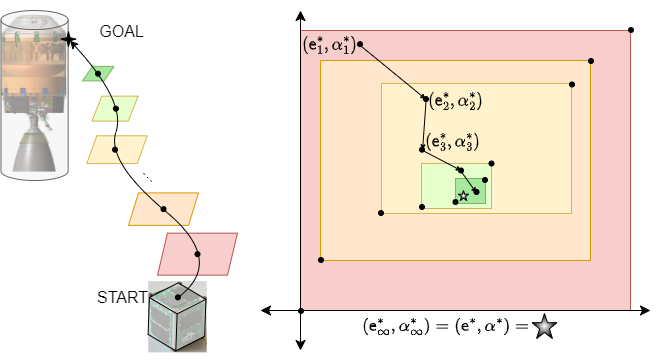
\includegraphics[width=0.95\linewidth]{assets/smid.png}
    \caption{Implementation of the Set Membership Identification (SMID) algorithm}
    \label{fig:smid}
\end{figure}
\begin{algorithm}
    \begin{algorithmic}[1]
        \small
        \Statex \textbf{Input:} $\boldsymbol{w}(\theta), \boldsymbol{u}(\theta) \text{ for } \theta\in[\theta_0,\theta_f]$, existing ${\mathcal{E}}$, ${\mathcal{A}}$; \, \textbf{Output:} updated ${\mathcal{E}}$, ${\mathcal{A}}$
        
        \State \underline{Generate a Feasible Solution Set (FSS)}
        \Statex \indent $\underline{{\mathsf{e}}}_{est} = \min{\mathsf{e}}$,
        \Statex \indent $\overline {{\mathsf{e}}}_{est} = \max{\mathsf{e}}$,
        \Statex \indent $\underline{ \alpha     }_{est} = \min{\alpha}$,
        \Statex \indent $\overline { \alpha     }_{est} = \max{\alpha}$, such that 
        \Statex \indent \indent $\boldsymbol{r}'=A(\theta; \alpha, \mathsf{e})\boldsymbol{r}+B(\theta; \alpha, \mathsf{e})\boldsymbol{u}+\boldsymbol{d}(\theta; \alpha, \mathsf{e})$,
        \Statex \indent \indent $\boldsymbol{p}(\theta_0)=\boldsymbol{w}(\theta_0)$, $||\boldsymbol{p}(\theta_f)-\boldsymbol{w}(\theta_f)||\leq D$,
        \Statex \indent \indent ${\mathsf{e}}\in{\mathcal{E}}$, $\alpha  \in{\mathcal{A}}$.
        
        \State \underline{Define the new FSS}
        \Statex \indent ${\mathcal{E}}_{new}={\mathcal{E}}\cap[\underline{{\mathsf{e}}}_{est}, \overline{{\mathsf{e}}}_{est}]$,
        \Statex \indent ${\mathcal{A}}_{new}={\mathcal{A}}\cap[\underline{\alpha}_{est},   \overline{\alpha}_{est}]$.
    
        \State \underline{Verify the new FSS}
        \Statex \indent Attempt to generate $\boldsymbol{r}(\theta)$ such that
        \Statex \indent \indent $\boldsymbol{r}'=A(\theta; \alpha, \mathsf{e})\boldsymbol{r}+B(\theta; \alpha, \mathsf{e})\boldsymbol{u}+\boldsymbol{d}(\theta; \alpha, \mathsf{e})$,
        \Statex \indent \indent $\boldsymbol{p}(\theta_0)=\boldsymbol{w}(\theta_0)$, $\boldsymbol{p}(\theta_f)\approx \boldsymbol{w}(\theta_f)$,
        \Statex \indent \indent ${\mathsf{e}}\in{\mathcal{E}}_{new}$, $\alpha  \in{\mathcal{A}}_{new}$.
    
        \State \underline{Compare and Update the FSS}
        \Statex \indent If Step 3 works:
        \Statex \indent \indent ${\mathcal{E}}\leftarrow{\mathcal{E}}_{new}$,
        \Statex \indent \indent ${\mathcal{A}}\leftarrow{\mathcal{A}}_{new}$.
        % \Statex \indent else: do nothing
        
        \State \underline{Update Data Range for Adaptation}
        \Statex \indent Consider new data by updating $\theta_0$ and $\theta_f$ as:
        \Statex \indent \indent $\Delta\theta = \theta_f - \theta_0$,
        \Statex \indent \indent $\theta_0 \leftarrow \theta_f$,
        \Statex \indent \indent $\theta_f \leftarrow \theta_f + \Delta \theta$.
    \end{algorithmic}
    \caption{A single iteration of \textbf{set membership identification (SMID)}}
    \label{alg:smid}
\end{algorithm}
We draw motivation from the idea of MSAC-MPC in \cite{tang2023indirect} to stop adaptation after a fixed number of iterations for computational simplicity.
We choose to stop adaptation at the end of rendezvous (before the start of docking) based on the shrunken size of the uncertainty tube.
The time or number of iterations for adaptation can be picked based on the accuracy of estimation.

We also assume that the intervals considered for the parameters are convex such that every value within two boundary values satisfies convex conditions.
This need not hold true when the intervals are large due to the nonlinear nature of the state space.
As a result, we recommend splitting the intervals such that each sub-interval is convex and treating the new FSS estimate as the union of all feasible sub-intervals.

\section{Summary}
This chapter focuses on the problem of chaser trajectory optimization to conduct rendezvous and docking to a point on the target.
A feasible trajectory is generated with cost minimization of the control effort and error from the final state while satisfying the relative motion dynamics of the chaser satellite in close proximity to the target in orbit.
This is followed by a discussion of the implementation of the set membership identification (SMID) algorithm to estimate the eccentricity of the orbit and the drag constant of the target.
The chapter also provides insight into the final state constraint that varies with time owing to the rotation of the target.
This involves convergence onto a rendezvous sphere followed by docking onto a predetermined point on the target.
This is followed by a discussion on the bounds of the states and the control inputs of the chaser.
The chapter ends by discussing the collision constraints associated with rendezvous and docking of which the latter is time-varying due to the rotation of the target.